\section*{Introduktion}
\label{Introduktion}
%
Formålet i denne rapport er at anvende metoden \textit{Multidimensional scaling (MDS)} til at analysere data indsamlet i en undersøgelse, hvor 13 forskellige ansigtsudtryk blev evalueret. Metoden MDS anvendes, da den kan bruges til at få indblik i hvilke faktorer der kan have haft betydning for vurderingen af ansigtsudtrykkene \parencite[p.2]{Wickelmaier2003}. De 13 ansigtsudtryk der blev undersøges er vist på \autoref{fig:ansigtsudtryk}. 

\begin{figure}[H]
\centering
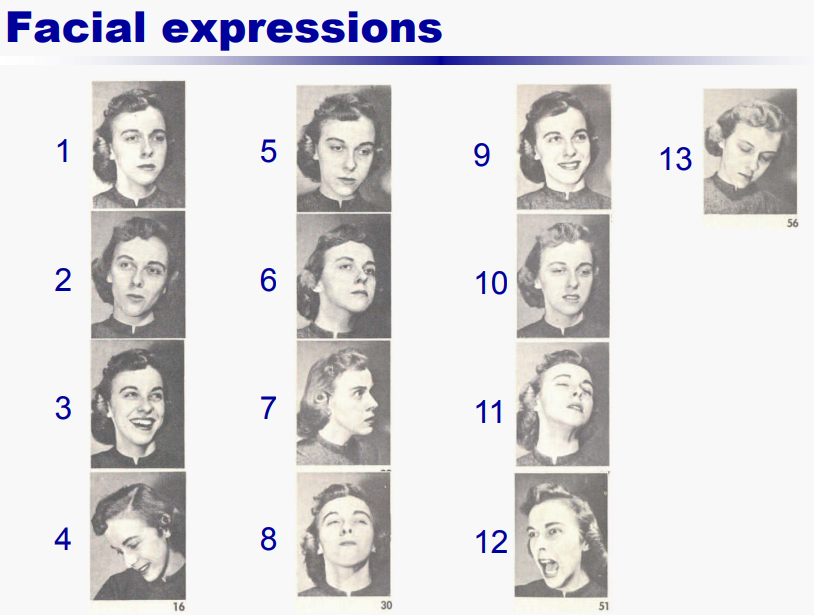
\includegraphics[width = 0.9\textwidth]{Figure/FacialExpressions.PNG} 
\caption{De 13 ansigtsudtryk der undersøges.}
\label{fig:ansigtsudtryk}
\end{figure}

%Analyses the data-set provided (using Matlab) (assume ordinal data).
%What type of MDS should you use? Argue for choice
%How many dimensions should you use? Plot scree plot
%How well a fit is your solution? Plot Shepard plot and interpret it
%Can you find meaningful dimensions? Label them.